\documentclass[conference]{IEEEtran}
\IEEEoverridecommandlockouts

\usepackage{cite}
\usepackage{amsmath,amssymb,amsfonts}
\usepackage{algorithm}
\usepackage{algpseudocode}
\usepackage{graphicx}
\usepackage{textcomp}
\usepackage{xcolor}
\usepackage{booktabs}
\usepackage{multirow}
\usepackage{tikz}
\usetikzlibrary{arrows.meta,positioning,fit,calc}
\usepackage[hidelinks]{hyperref}
\usepackage{url}

\graphicspath{{figures/}}
\newcommand{\code}[1]{\texttt{\small #1}}

\begin{document}

\title{CRS: A Fine-Tuned Small Transformer for Evidence-Grounded Clinical Trial Criterion Screening with KV Caching, Tiled Attention and Speculative Decoding}

\author{\IEEEauthorblockN{Huma Taj}
\IEEEauthorblockA{\textit{Roll No. 23i-0743} \\
\textit{Department of Computer Science}\\
\textit{National University of Computer and Emerging Sciences (FAST-NUCES)}\\
Islamabad, Pakistan \\
i230743@isb.nu.edu.pk}}

\maketitle

\begin{abstract}
Matching patients to clinical trials requires judging every inclusion and exclusion criterion against a free-text patient record and justifying each judgement. We present CRS (Clinical Records Screener), a complete, locally executable system built on the open-weight Qwen2.5-1.5B-Instruct decoder and adapted with Low-Rank Adaptation (LoRA) on the TrialGPT Criterion Annotations dataset. Given a numbered patient note, a criterion type and the criterion text, the model emits a JSON object containing one of the expert label categories (including \emph{not enough information} and \emph{not applicable}) and the IDs of supporting patient sentences. On a fixed, patient-grouped held-out test split (8 patients, 206 criteria), fine-tuning raised accuracy from 0.204 to 0.728, macro-F1 from 0.234 to 0.560 and evidence micro-F1 from 0.130 to 0.523, with no invalid outputs. We also implement, from model forward passes upward, (i) an explicit KV-cached greedy decoder that matches a full-recompute reference token for token in all nine tested input/output lengths and keeps throughput flat at about 25 tokens/s while the reference falls to 2.8 tokens/s; (ii) a tiled online-softmax attention whose maximum error against reference attention stays below $1.4\times10^{-6}$ and which reduces peak GPU memory at length 4096 from 1536\,MB to 18\,MB; and (iii) greedy speculative decoding with a fine-tuned Qwen2.5-0.5B draft that reproduces greedy output exactly but runs 0.51--0.85$\times$ as fast on a Tesla T4, a slowdown we explain with measured draft, verification and synchronisation costs. All components are exposed through a browser application that screens unseen notes, highlights evidence and exports a report.
\end{abstract}

\begin{IEEEkeywords}
clinical trial matching, large language models, LoRA, evidence retrieval, KV cache, online softmax, speculative decoding
\end{IEEEkeywords}

%=====================================================================
\section{Introduction}
%=====================================================================
Recruiting patients is a major bottleneck in clinical research, and manual pre-screening of eligibility criteria is slow and labour-intensive \cite{jin2024trialgpt}. Each trial lists inclusion criteria a patient must meet and exclusion criteria a patient must not meet; each criterion must be compared with an unstructured clinical note. TrialGPT \cite{jin2024trialgpt} showed that a proprietary large language model (GPT-4) can make these criterion-level judgements and cite supporting sentences. Proprietary APIs are, however, costly, cannot be inspected, and raise privacy concerns for clinical text.

This work asks whether a \emph{small, open-weight} Transformer that runs on free or consumer hardware can be adapted to the same criterion-level task, while remaining transparent about its evidence. The problem is defined as follows. Given a patient note split into numbered sentences $S=\{s_0,\dots,s_{n-1}\}$, a criterion type $t\in\{\text{inclusion},\text{exclusion}\}$ and criterion text $c$, predict a label $y$ from the expert label set for $t$ and a subset $E\subseteq\{0,\dots,n-1\}$ of sentence IDs that support $y$. The four inclusion labels are \emph{included}, \emph{not included}, \emph{not enough information} and \emph{not applicable}; the exclusion labels replace the first two with \emph{excluded} and \emph{not excluded}. These categories are preserved and are never collapsed into a binary decision.

Our contributions are:
\begin{enumerate}
\item A reproducible fine-tuning pipeline on a prescribed patient-grouped split, with a before/after comparison of the same model under identical greedy decoding (Sections~\ref{sec:data}--\ref{sec:finetune}).
\item Criterion and evidence evaluation with per-class metrics, confusion matrices, explicit empty-set rules, patient-level bootstrap intervals and an analysis of twelve distinct errors (Sections~\ref{sec:eval}, \ref{sec:results}).
\item From-scratch implementations of KV-cached decoding, tiled online-softmax attention and greedy speculative decoding, each verified for exact or numerically bounded equivalence and benchmarked with warm-up and synchronised repeated timing (Section~\ref{sec:inference}).
\item A browser application that runs the fine-tuned model on unseen notes, shows the cited evidence for every criterion, exposes live decoding and attention comparisons, and exports a report with model provenance (Section~\ref{sec:app}).
\end{enumerate}

%=====================================================================
\section{Related Work}
%=====================================================================
\textbf{Patient--trial matching.} TrialGPT \cite{jin2024trialgpt} decomposes matching into criterion-level prediction, trial-level aggregation and ranking, using GPT-4 with chain-of-thought explanations and sentence-level evidence. Its released Criterion Annotations dataset \cite{trialgptdataset}, with expert labels and expert evidence sentences, is the benchmark used here. TrialGPT relies on a closed model; we study whether a 1.5B-parameter open model can learn the criterion-level task directly from expert labels, without using any GPT-4 output as input or target.

\textbf{Transformer decoders.} The Transformer \cite{vaswani2017attention} computes scaled dot-product attention $\mathrm{softmax}(QK^\top/\sqrt{d})V$; decoder-only variants generate autoregressively under a causal mask. Qwen2.5 \cite{qwen2025qwen25} adds rotary position embeddings (RoPE), grouped-query attention (GQA), SwiGLU feed-forward blocks and RMSNorm. Qwen3 \cite{qwen2025qwen3} introduces a default ``thinking'' mode that emits reasoning text before the answer, and SmolLM2 \cite{allal2025smollm2} is a data-centric 1.7B model trained largely on English web and code.

\textbf{Parameter-efficient fine-tuning.} LoRA \cite{hu2022lora} freezes pretrained weights and learns a low-rank update $\Delta W = BA$ with $B\in\mathbb{R}^{d\times r}$, $A\in\mathbb{R}^{r\times k}$, $r\ll\min(d,k)$, cutting trainable parameters by orders of magnitude. QLoRA \cite{dettmers2023qlora} further quantises the frozen weights to 4 bits. With only 602 training rows, full fine-tuning would overfit and require far more memory, so we use LoRA; QLoRA was unnecessary because the 1.5B model fits in 16-bit precision on a free Tesla T4.

\textbf{Efficient attention.} The online normaliser of Milakov and Gimelshein \cite{milakov2018online} computes softmax in one pass with a running maximum and sum. FlashAttention \cite{dao2022flashattention} combines this with tiling so that the $N\times N$ score matrix is never materialised in GPU high-bandwidth memory, giving exact attention with linear extra memory. Its speed comes from a fused CUDA kernel; an educational PyTorch version keeps the memory benefit but not the fusion.

\textbf{Speculative decoding.} Leviathan \emph{et al.} \cite{leviathan2023fast} and Chen \emph{et al.} \cite{chen2023accelerating} let a small draft model propose $k$ tokens that the large target verifies in one forward pass; with greedy acceptance the output is identical to the target's greedy output. Speedup depends on the acceptance rate and on the draft being much cheaper than the target, which our measurements test directly.

%=====================================================================
\section{Materials and Methods}
%=====================================================================
\subsection{Dataset and Split}\label{sec:data}
The TrialGPT Criterion Annotations dataset \cite{trialgptdataset} (revision \code{1cfcafd}) has 1{,}015 criterion-level rows from 53 patients (TREC/SIGIR cohorts). Each row holds a numbered patient note, a trial ID, the criterion type and text, an expert eligibility label and expert evidence sentence IDs. It also contains GPT-4 labels, sentences and explanations; our loader reads an explicit allow-list of eight columns so that no \code{gpt4\_*} or \code{explanation\_correctness} value can reach a prompt or target, which a unit test enforces.

Following the common protocol, unique patient IDs are sorted, shuffled with \code{numpy.random.default\_rng(42)}, and the first 37 assigned to training, the next 8 to validation and the last 8 to test. The dataset's own \code{training} column is ignored. One row (annotation 883) has a blank criterion and was removed before any experiment; it remains in the manifest totals. Table~\ref{tab:split} summarises the split; the published manifest (\code{splits/manifest.json}) lists every patient ID and per-patient row counts, and tests assert that the three patient sets are disjoint, cover all 53 patients and are reproducible.

\begin{table}[t]
\centering
\caption{Patient-grouped split (seed 42) and label counts.}
\label{tab:split}
\setlength{\tabcolsep}{4pt}
\begin{tabular}{lrrr}
\toprule
 & Train & Validation & Test \\
\midrule
Patients & 37 & 8 & 8 \\
Usable rows & 602 & 206 & 206 \\
\midrule
Incl.\ / included & 88 & 35 & 27 \\
Incl.\ / not included & 13 & 3 & 7 \\
Incl.\ / not enough information & 109 & 27 & 38 \\
Incl.\ / not applicable & 5 & 1 & 3 \\
Excl.\ / excluded & 8 & 2 & 0 \\
Excl.\ / not excluded & 291 & 101 & 91 \\
Excl.\ / not enough information & 65 & 26 & 28 \\
Excl.\ / not applicable & 23 & 11 & 12 \\
\bottomrule
\end{tabular}
\end{table}

The label distribution is heavily skewed: \emph{excluded} has 8 training rows and none in test, and \emph{not included} has 13. Evidence is often empty: 610 of 1{,}015 rows have no expert evidence, including 74.7\% of training rows labelled \emph{not excluded}, because annotators frequently concluded ``not excluded'' when a condition was never mentioned. This tension with the requirement that absent evidence must not count as proof is handled in the application (Section~\ref{sec:app}) rather than by altering labels.

\subsection{Input and Output Format}
Each example is rendered with the model's chat template. The system message instructs the model to use only the numbered note and reply with one JSON object. The user message contains the note as lines \code{[i] sentence}, the criterion type with definitions of its four labels, and the criterion text. The target is \code{\{"label": "<label>", "evidence": [ids]\}}. The training loss covers only the assistant's answer tokens. A verifier parses the output, checks the label is legal for the criterion type and that every cited ID exists; any violation counts as an invalid prediction and is reported as a separate rate.

\textbf{Truncation.} Prompts were tokenised with the Qwen2.5 tokenizer and never truncated. The longest note is 372 tokens and the longest full prompt 634 tokens (train median 318, 95th percentile 506; validation maximum 468), far below the 32{,}768-token context window, so no patient evidence is removed (\code{results/truncation.json}).

\subsection{Model Selection}
Table~\ref{tab:models} compares the candidates. All three are Apache-2.0 licensed decoder-only models. Qwen2.5-1.5B-Instruct was selected because (i) it reached the highest validation macro-F1 after identical fine-tuning (Section~\ref{sec:finetune}); (ii) GQA with only two key/value heads keeps the KV cache at 28\,KB per token in float16 ($28\text{ layers}\times2\times2\text{ heads}\times128\times2$ bytes); (iii) at about 3.1\,GB in float16 it fits a 4\,GB laptop GPU for inference and a 16\,GB T4 for training; and (iv) Qwen2.5-0.5B-Instruct shares its vocabulary (151{,}665 tokens), special tokens, chat template and encodings exactly, which we verified programmatically and which speculative decoding requires. Qwen3 was rejected because its default thinking mode complicates strict JSON output and its 4B model (about 8\,GB in float16) does not fit the development GPU. SmolLM2-1.7B was trained as a competitor (run R5).

\begin{table}[t]
\centering
\caption{Candidate open-weight decoder models.}
\label{tab:models}
\setlength{\tabcolsep}{3pt}
\begin{tabular}{lccc}
\toprule
 & Qwen2.5-1.5B & SmolLM2-1.7B & Qwen2.5-0.5B \\
 & (target) & (candidate) & (draft) \\
\midrule
Parameters & 1{,}543.7M & 1{,}711.4M & 494.0M \\
Layers & 28 & 24 & 24 \\
Hidden size & 1536 & 2048 & 896 \\
Q / KV heads & 12 / 2 & 32 / 32 & 14 / 2 \\
Context & 32{,}768 & 8{,}192 & 32{,}768 \\
Tokenizer & Qwen2 BPE & SmolLM2 BPE & = target \\
fp16 weights & 3.1\,GB & 3.4\,GB & 1.0\,GB \\
License & Apache-2.0 & Apache-2.0 & Apache-2.0 \\
\bottomrule
\end{tabular}
\end{table}

\subsection{Fine-Tuning}\label{sec:finetune}
We use LoRA \cite{hu2022lora} via PEFT \cite{peft} on the query, key, value and output projections of every attention layer, with dropout 0.05. Training uses AdamW at learning rate $2\times10^{-4}$ with 10\% linear warm-up, gradient clipping at 1.0, batch size 4 with 2 accumulation steps (8 examples per update), gradient checkpointing, seed 42, up to 10 epochs and early stopping with patience 2 on validation macro-F1 computed from real greedy generation (not loss). Rare labels can be oversampled with weight proportional to $(\text{count})^{-p}$.

Table~\ref{tab:runs} lists the experiment grid, all evaluated on validation only. Selection was fixed in advance: highest validation macro-F1 among Qwen2.5-1.5B runs, then evidence F1. R3 (rank 32, $\alpha=64$, oversampling $p=0.5$; about 8.7M trainable parameters, 0.57\% of the model) was chosen. Training took 1{,}295\,s on a Kaggle Tesla T4 with 7.55\,GB peak memory. Fig.~\ref{fig:curves}(a) shows that validation loss bottoms out at epoch 3 while training loss keeps falling; Fig.~\ref{fig:curves}(b) shows that validation macro-F1 peaks later (epoch 4, 0.558), which is why early stopping uses the generated metric rather than loss. With only 8 validation patients the 95\% bootstrap interval for R3's macro-F1 is 0.42--0.64, so R1--R3 are statistically indistinguishable; R3 is selected by the pre-stated rule. Listing evidence before the label (R4) improved evidence F1 but cut macro-F1 to 0.459, so the label-first order was kept.

\begin{table}[t]
\centering
\caption{Fine-tuning runs, validation split (206 rows).}
\label{tab:runs}
\setlength{\tabcolsep}{3pt}
\begin{tabular}{llcccc}
\toprule
Run & Setting & Acc. & Macro-F1 & Evid.\ F1 & Epoch \\
\midrule
R0 & Qwen-1.5B, untrained & 0.175 & 0.147 & 0.106 & -- \\
R0b & SmolLM2, untrained & 0.180 & 0.120 & 0.111 & -- \\
R1 & LoRA $r$=16 & 0.752 & 0.534 & 0.462 & 3 \\
R2 & $r$=16, oversample & 0.738 & 0.552 & 0.487 & 4 \\
\textbf{R3} & \textbf{$r$=32, oversample} & \textbf{0.743} & \textbf{0.558} & \textbf{0.509} & 4 \\
R4 & R3, evidence first & 0.762 & 0.459 & 0.526 & 7 \\
R5 & SmolLM2, R3 config & 0.675 & 0.514 & 0.446 & 2 \\
R6 & Qwen-0.5B, R3 config & 0.738 & 0.446 & 0.491 & 2 \\
\bottomrule
\end{tabular}
\end{table}

\begin{figure*}[t]
\centering
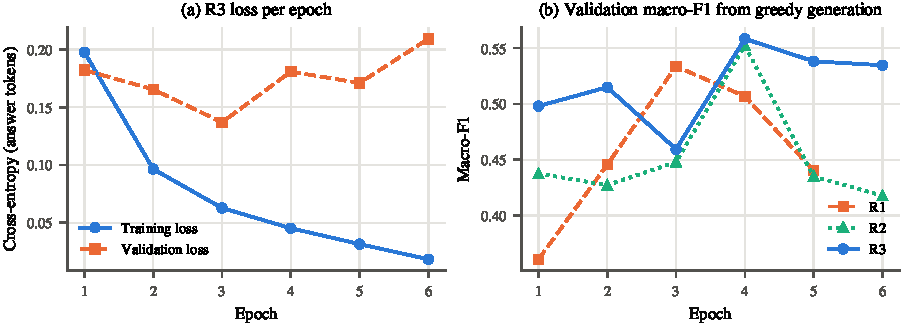
\includegraphics[width=\textwidth]{training_curves}
\caption{Training dynamics. (a) R3 answer-token cross-entropy: validation loss is lowest at epoch 3 and rises afterwards while training loss keeps falling, an early sign of overfitting on 602 rows. (b) Validation macro-F1 from greedy generation for R1--R3; R3 peaks at 0.558 in epoch 4. Loss and generated macro-F1 do not move together, so early stopping uses macro-F1.}
\label{fig:curves}
\end{figure*}

\textbf{Explanations.} The only written explanations in the dataset are GPT-4's, which the protocol bars, so the model is not trained to explain. We tested asking the base model to paraphrase a verdict from the cited sentences only; on validation rows it invented facts (calling a female patient male, and stating that age 58 lies outside 25--65). Explanations are therefore templated: they state the verdict and quote the cited sentences verbatim, so they cannot introduce a fact.

\subsection{System Architecture}
Fig.~\ref{fig:arch} shows the end-to-end pipeline used by both evaluation and the application.

\begin{figure*}[t]
\centering
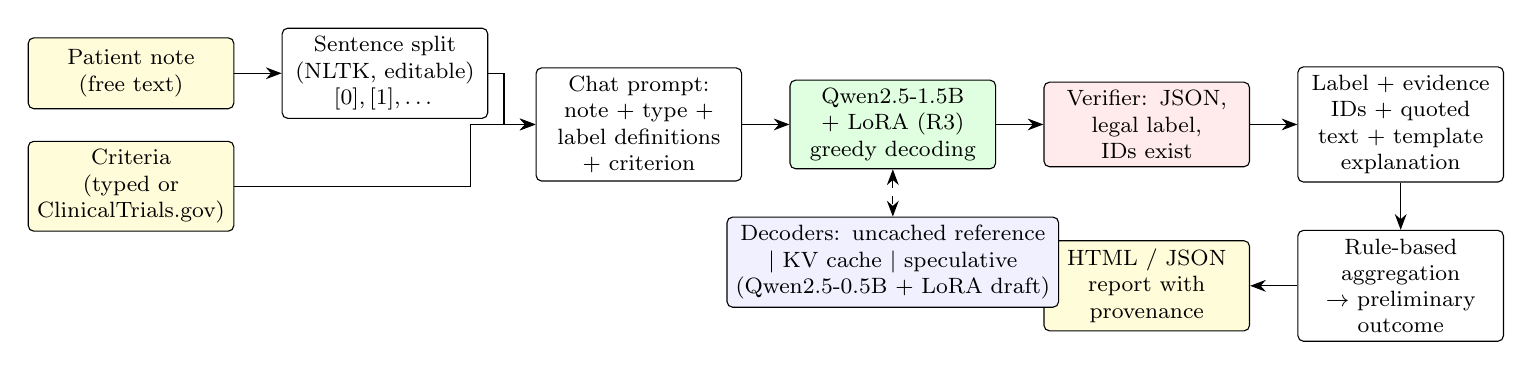
\begin{tikzpicture}[
  node distance=4mm and 6mm,
  box/.style={draw, rounded corners=2pt, align=center, font=\footnotesize, minimum height=9mm, inner sep=3pt, text width=24mm},
  data/.style={box, fill=yellow!15},
  model/.style={box, fill=green!12},
  check/.style={box, fill=red!8},
  >={Stealth[length=2mm]}]
\node[data] (note) {Patient note\\(free text)};
\node[box, right=of note] (split) {Sentence split\\(NLTK, editable)\\$[0],[1],\dots$};
\node[data, below=of note] (crit) {Criteria\\(typed or\\ClinicalTrials.gov)};
\node[box, right=of split, yshift=-6.5mm] (prompt) {Chat prompt:\\note + type +\\label definitions\\+ criterion};
\node[model, right=of prompt] (llm) {Qwen2.5-1.5B\\+ LoRA (R3)\\greedy decoding};
\node[check, right=of llm] (verify) {Verifier: JSON,\\legal label,\\IDs exist};
\node[box, right=of verify] (out) {Label + evidence\\IDs + quoted\\text + template\\explanation};
\node[box, below=of out, yshift=-2mm] (agg) {Rule-based\\aggregation\\$\rightarrow$ preliminary\\outcome};
\node[data, left=of agg] (report) {HTML / JSON\\report with\\provenance};
\node[box, below=of llm, yshift=-2mm, text width=40mm, fill=blue!6] (dec) {Decoders: uncached reference $|$ KV cache $|$ speculative (Qwen2.5-0.5B + LoRA draft)};
\draw[->] (note) -- (split);
\draw[->] (split.east) -- ++(2mm,0) |- (prompt.west);
\draw[->] (crit.east) -- ++(30mm,0) |- (prompt.west);
\draw[->] (prompt) -- (llm);
\draw[->] (llm) -- (verify);
\draw[->] (verify) -- (out);
\draw[->] (out) -- (agg);
\draw[->] (agg) -- (report);
\draw[<->, dashed] (llm) -- (dec);
\end{tikzpicture}
\caption{CRS pipeline. Each criterion is judged independently by the fine-tuned model under one of three interchangeable decoders; the verifier rejects malformed or illegal outputs; criterion results are aggregated by an explicit rule into a preliminary, non-ground-truth outcome.}
\label{fig:arch}
\end{figure*}

%=====================================================================
\section{Inference Mechanisms}\label{sec:inference}
%=====================================================================
All three mechanisms are written as explicit loops over model forward passes (\code{screener/inference/}, \code{screener/attention/}); library generation APIs are used only as a third, independent correctness check.

\subsection{KV-Cached Greedy Decoding}
The reference decoder recomputes the full sequence at every step with caching disabled, costing $O(T^2)$ token-layer work for $T$ tokens. The cached decoder (Algorithm~\ref{alg:kv}) runs the prompt once (\emph{prefill}), storing each layer's keys and values, and then feeds only the newest token per step (\emph{decode}).

\begin{algorithm}[t]
\caption{Explicit KV-cached greedy decoding}\label{alg:kv}
\begin{algorithmic}[1]
\Require prompt ids $x_{1:L}$, mask $m_{1:L}$, limit $N$, EOS set
\State $\mathcal{C}\gets$ empty cache; $p\gets \mathrm{cumsum}(m)-1$ \Comment{positions from mask}
\State $z\gets f(x_{1:L}, m, p, \mathcal{C})$ \Comment{prefill; fills $\mathcal{C}$}
\State assert $|\mathcal{C}|=L$; $y\gets\arg\max z_L$; out $\gets[y]$
\While{$y\notin$ EOS \textbf{and} $|\text{out}|<N$}
  \State $m\gets[m,1]$; $p\gets p_{\text{last}}+1$
  \State $z\gets f(y, m, p, \mathcal{C})$ \Comment{one token; appends to $\mathcal{C}$}
  \State assert $|\mathcal{C}|=L+|\text{out}|$; $y\gets\arg\max z$; append $y$
\EndWhile
\end{algorithmic}
\end{algorithm}

\textbf{Positions.} RoPE rotates queries and keys by their absolute position, so the new token must receive position $p_{\text{last}}+1$, not 0. Positions are derived from the attention mask ($\mathrm{cumsum}(m)-1$), which makes left-padded prompts correct; a test confirms identical output with and without left padding. \textbf{Masking.} The decode step's single query may attend to every cached key, so the causal constraint is satisfied automatically; the mask is extended by one column per step so that padding stays hidden. \textbf{Cache growth.} The cache grows linearly by 28\,KB per token (float16), from 1.75\,MB after a 64-token prefill to 35.0\,MB after 1{,}024 + 256 tokens (Fig.~\ref{fig:kv}b); the decoder asserts the cache length after every step. \textbf{Numerical differences.} Cached and uncached paths reduce the same dot products in different orders and with different matrix shapes, so float16 logits can differ slightly; the largest observed difference was 0.168, never enough to change an $\arg\max$.

\subsection{Tiled Attention with Online Softmax}
The reference computes $S=QK^\top/\sqrt{d}$, sets masked entries to $-\infty$, subtracts the row maximum, exponentiates, normalises and multiplies by $V$, guarding fully masked rows. The tiled version (Algorithm~\ref{alg:tile}) visits query tiles and key tiles of size $B$, keeping per row a running maximum $m$, normaliser $\ell$ and unnormalised output $O$; whenever $m$ increases, previous $\ell$ and $O$ are rescaled by $e^{m_{\text{old}}-m_{\text{new}}}$ \cite{milakov2018online,dao2022flashattention}. Key tiles lying entirely above the causal diagonal are skipped; at length 4096 with $B=256$, 120 of 256 tiles are never computed. No fused backend is called. A model patch swaps this function into every attention layer of Qwen2.5-0.5B, and a unit test confirms that generation then produces identical tokens.

\begin{algorithm}[t]
\caption{Tiled online-softmax attention (per head)}\label{alg:tile}
\begin{algorithmic}[1]
\For{each query tile $Q_i$}
  \State $m\gets-\infty$, $\ell\gets 0$, $O\gets 0$
  \For{each key tile $j$ not fully above the diagonal}
    \State $S\gets Q_iK_j^\top/\sqrt d$; apply causal/padding mask
    \State $m'\gets\max(m,\mathrm{rowmax}(S))$; $P\gets e^{S-m'}$
    \State $\ell\gets e^{m-m'}\ell+\mathrm{rowsum}(P)$
    \State $O\gets e^{m-m'}O+PV_j$; $m\gets m'$
  \EndFor
  \State output$_i\gets O/\ell$ \Comment{rows with $\ell=0$ return 0}
\EndFor
\end{algorithmic}
\end{algorithm}

\subsection{Greedy Speculative Decoding}
Target and draft are Qwen2.5-1.5B (+R3 adapter) and Qwen2.5-0.5B (+R6 adapter), whose tokenizers are identical. Both caches obey one invariant, asserted every round: \emph{each cache holds every token of the sequence except the last}. One round (Algorithm~\ref{alg:spec}) drafts up to $k$ tokens, verifies them with one target pass over the last token plus the $k$ candidates, accepts the longest matching prefix, appends the target's own token as a correction (or as a bonus if all $k$ matched), and crops both caches back to the accepted length. EOS and the length limit are handled mid-round. Because every emitted token is the target's greedy choice, the output must equal greedy decoding exactly; tests cover all-accepted, all-rejected and EOS-inside-draft rounds, and Hugging Face assisted generation is used only as a reference check.

\begin{algorithm}[t]
\caption{One round of greedy speculative decoding}\label{alg:spec}
\begin{algorithmic}[1]
\Require sequence $x$; caches $\mathcal{C}_T,\mathcal{C}_D$ hold $x_{1:|x|-1}$
\State draft $d_{1:k}$ greedily with the draft model from $x_{|x|}$
\State $g_{0:k}\gets\arg\max f_T([x_{|x|},d_{1:k}],\mathcal{C}_T)$ \Comment{one pass}
\State $a\gets$ largest $a$ with $d_{1:a}=g_{0:a-1}$
\State append $d_{1:a}$ and $g_a$ to $x$ \Comment{correction or bonus}
\State crop $\mathcal{C}_T,\mathcal{C}_D$ to $|x|-1$ tokens; feed draft any unread token
\end{algorithmic}
\end{algorithm}

%=====================================================================
\section{Application}\label{sec:app}
%=====================================================================
The application is a FastAPI server that loads the model once and serves a React interface at \url{http://127.0.0.1:8600}; it is started with one command (\code{./start\_app.sh} or \code{start\_app.bat}) and needs no notebook or IDE. The workflow is: (1) paste, upload or load a sample note; (2) review and correct the numbered sentences; (3) enter criteria or import them from ClinicalTrials.gov by NCT number, and choose a decoder; (4) inspect results (Fig.~\ref{fig:app}). Every screen shows the notice ``Educational screening prototype. Not a clinical enrollment decision.''

The overall outcome is an explicit rule, not a learned label: \emph{Likely ineligible} if any criterion fails \emph{with cited evidence}; otherwise \emph{Needs review} if any verdict is unknown, unverified or uncited; otherwise \emph{Potentially eligible}. Requiring citations means a silent note can never by itself make a patient ineligible or eligible. A model lab runs the three decoders and the two attention implementations live on the current machine and reports token equality, timings, acceptance and memory, and saved reports can be reopened. Reports record the note hash, decoding mode and the exact Hugging Face revisions of the base model and adapter. Inputs are validated (empty, oversized or non-text notes, empty sentences, missing criteria, illegal modes) with readable messages, and a deterministic number check corrects bare numeric comparisons when the note contains one clear value; it was validated on training and validation data only and never run on the test split.

\begin{figure*}[t]
\centering
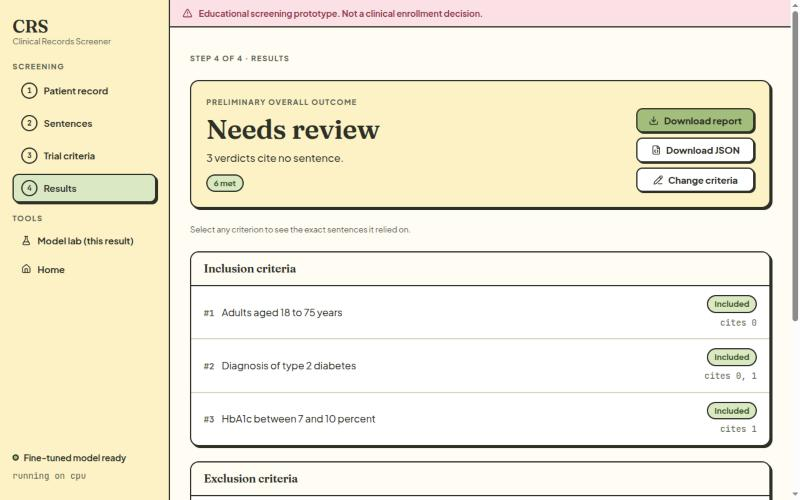
\includegraphics[width=0.49\textwidth]{app_results.jpg}\hfill
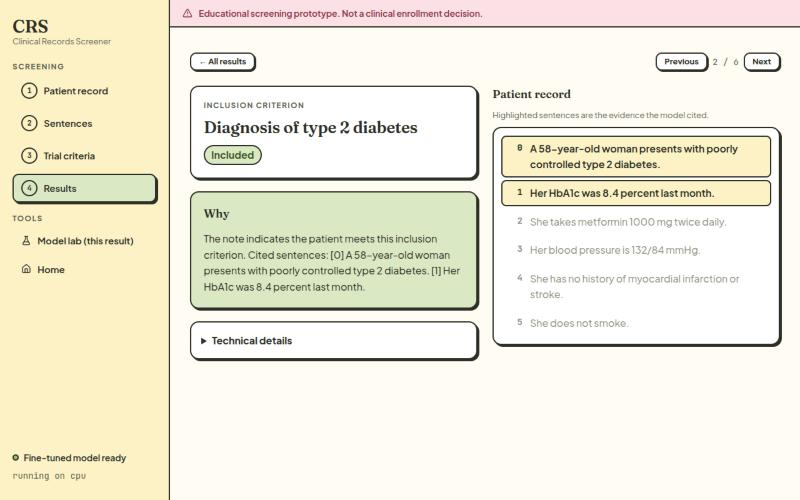
\includegraphics[width=0.49\textwidth]{app_evidence.jpg}\\[2mm]
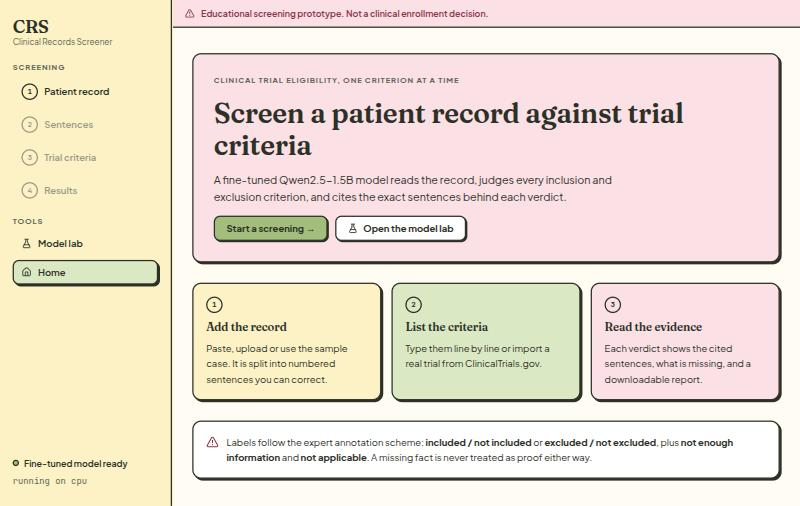
\includegraphics[width=0.49\textwidth]{app_home.jpg}\hfill
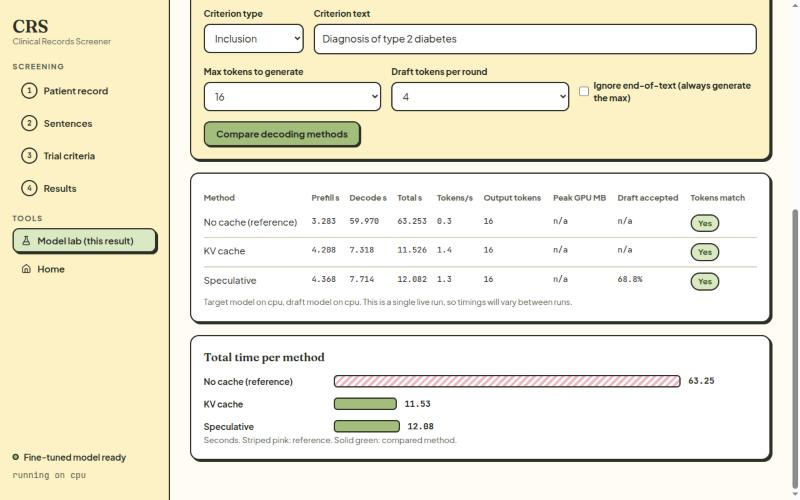
\includegraphics[width=0.49\textwidth]{app_lab.jpg}
\caption{Browser application running on a CPU-only laptop. Top left: preliminary outcome, count chips, report export and per-criterion verdicts with cited sentence IDs. Top right: one criterion with its verdict, templated explanation and the cited sentences highlighted in the note. Bottom left: home screen with the persistent prototype notice. Bottom right: live decoding comparison; all three decoders produce the same 16 tokens, and KV caching cuts total time from 63.3\,s to 11.5\,s.}
\label{fig:app}
\end{figure*}

%=====================================================================
\section{Experimental Setup and Metrics}\label{sec:eval}
%=====================================================================
\textbf{Hardware.} Training and the reported benchmarks used a free Kaggle Tesla T4 (16\,GB, PyTorch 2.11 \cite{paszke2019pytorch}, Transformers 5.8 \cite{wolf2020transformers}). Development used a laptop with an RTX 3050 Ti (4\,GB); the demonstration runs on a CPU-only laptop (8 threads, 15\,GB RAM) with float32 weights.

\textbf{Decoding.} All evaluations use greedy decoding (no sampling, one beam, repetition penalty 1.0, at most 96 new tokens); Qwen's bundled sampling defaults are overridden explicitly. Before and after fine-tuning use identical prompts, examples and settings.

\textbf{Classification metrics.} Accuracy, macro-F1 and per-class precision, recall and F1, with confusion matrices, overall and separately for inclusion and exclusion criteria. Labels with no gold examples in a split are reported as n/a and excluded from macro-F1; the variant that counts them as zero is also given. Invalid outputs count as wrong.

\textbf{Evidence metrics.} Micro precision/recall/F1 over all (row, sentence) pairs, and macro averages per row. Empty sets: both empty counts as perfect in the all-rows macro score; gold empty with predictions gives precision 0; gold present with no prediction gives recall 0. We report the macro score both on all rows and on the rows that have gold evidence.

\textbf{Uncertainty and baselines.} 95\% intervals use a patient-level bootstrap (2{,}000 resamples, seed 42), since rows of one patient are correlated. Baselines are a majority-label predictor per criterion type that cites nothing. \textbf{Test access.} The evaluator refuses the test split unless called with \code{--final}, and logs each access; the configuration was tagged \code{final-config} before the single test evaluation.

\textbf{Benchmarks.} Each configuration is preceded by discarded warm-up runs, timed with \code{torch.cuda.synchronize()} around each interval, repeated five times, and reported as the median. Peak memory is measured as the GPU allocation above the loaded model weights.

%=====================================================================
\section{Results and Discussion}\label{sec:results}
%=====================================================================
\subsection{Criterion Classification}
Fig.~\ref{fig:beforeafter} and Table~\ref{tab:test} compare the same model before and after fine-tuning on the held-out test split. The untrained model is worse than always predicting the majority label in accuracy (0.204 vs 0.626) because it spreads predictions across categories without regard to the note. Fine-tuning raises accuracy to 0.728 (95\% CI 0.60--0.83) and macro-F1 to 0.560 (CI 0.43--0.64), well above the baseline's 0.272. Test results are close to validation (0.743 / 0.558), indicating no selection overfitting. No output was invalid and no cited ID was out of range.

\begin{figure}[t]
\centering
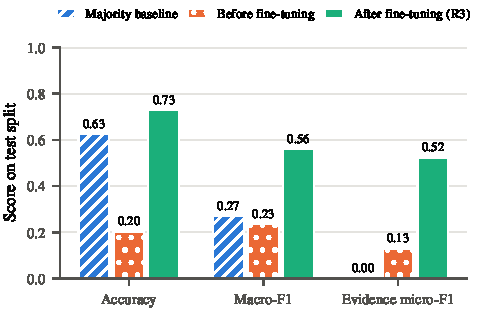
\includegraphics[width=\columnwidth]{before_after}
\caption{Test-split comparison of the majority baseline and Qwen2.5-1.5B before and after LoRA fine-tuning, with identical greedy decoding. The baseline's accuracy is high only because the label distribution is skewed; its macro-F1 and evidence F1 are low.}
\label{fig:beforeafter}
\end{figure}

\begin{table}[t]
\centering
\caption{Held-out test results (8 patients, 206 criteria).}
\label{tab:test}
\setlength{\tabcolsep}{3.5pt}
\begin{tabular}{llccc}
\toprule
Subset & System & Acc. & Macro-F1 & Evid.\ $\mu$F1 \\
\midrule
\multirow{3}{*}{Overall (206)} & Majority & 0.626 & 0.272 & 0.000 \\
 & Before & 0.204 & 0.234 & 0.130 \\
 & \textbf{After} & \textbf{0.728} & \textbf{0.560} & \textbf{0.523} \\
\midrule
\multirow{2}{*}{Inclusion (75)} & Before & 0.267 & 0.203 & 0.260 \\
 & After & 0.773 & 0.469 & 0.631 \\
\midrule
\multirow{2}{*}{Exclusion (131)} & Before & 0.168 & 0.170 & 0.085 \\
 & After & 0.702 & 0.427 & 0.190 \\
\bottomrule
\end{tabular}
\end{table}

Table~\ref{tab:perclass} and Fig.~\ref{fig:confusion} break results down by class. \emph{Included} is predicted with precision 1.00, and \emph{not excluded} with recall 0.96. The two weaknesses are complementary. On exclusion criteria the model defaults to \emph{not excluded}: 24 of 28 exclusion \emph{not enough information} rows and 8 of 12 \emph{not applicable} rows are predicted that way, which mirrors the training data, where most \emph{not excluded} rows cite nothing. On inclusion criteria it retreats to \emph{not enough information} when the answer needs a clinical inference, so that label has recall 1.00 while \emph{not included} has recall 0.14 (1 of 7). \emph{Excluded} has no test rows, so its performance cannot be measured on this split; macro-F1 counting it as zero is 0.466.

\begin{table}[t]
\centering
\caption{Per-class test metrics after fine-tuning (all criteria).}
\label{tab:perclass}
\setlength{\tabcolsep}{4pt}
\begin{tabular}{lcccc}
\toprule
Label & Support & Precision & Recall & F1 \\
\midrule
included & 27 & 1.000 & 0.704 & 0.826 \\
not included & 7 & 0.500 & 0.143 & 0.222 \\
excluded & 0 & n/a & n/a & n/a \\
not excluded & 91 & 0.731 & 0.956 & 0.829 \\
not enough information & 66 & 0.667 & 0.606 & 0.635 \\
not applicable & 15 & 0.500 & 0.200 & 0.286 \\
\bottomrule
\end{tabular}
\end{table}

\begin{figure*}[t]
\centering
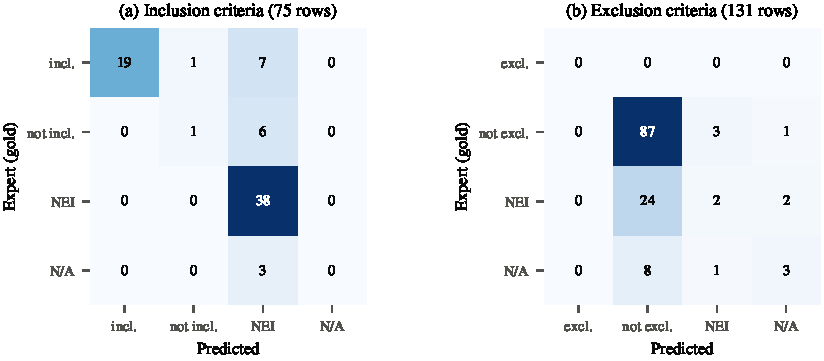
\includegraphics[width=0.82\textwidth]{confusion}
\caption{Test confusion matrices after fine-tuning (rows: expert label; NEI: not enough information; N/A: not applicable). (a) On inclusion criteria, errors flow into NEI when inference is needed. (b) On exclusion criteria, 32 of 40 NEI and N/A rows are predicted as ``not excluded''.}
\label{fig:confusion}
\end{figure*}

\subsection{Evidence Localisation}
Evidence micro-F1 rose from 0.130 to 0.523 (precision 0.577, recall 0.479; CI 0.41--0.64). The untrained model over-cites (micro precision 0.078). Of the 206 test rows, 136 have empty gold and empty predictions, 37 have both non-empty, 24 have gold evidence but no prediction, and 9 cite sentences where the gold has none. Macro-F1 is 0.817 over all rows, inflated by the both-empty rows, and 0.528 over the 61 rows that have gold evidence, which is the more informative figure. Inclusion evidence is much better (micro-F1 0.631) than exclusion evidence (0.190), consistent with the model's habit of answering \emph{not excluded} without a citation.

\subsection{Error Analysis}
Twelve distinct test errors were analysed (\code{results/error_analysis.md}); Table~\ref{tab:errors} summarises them. Seventeen of the 24 rows in the largest error cell (gold NEI, predicted not excluded) come from one patient on one trial, showing how much a single annotator's convention can move totals on an 8-patient split. Two gold labels for the same situation (a pregnancy criterion for a male patient) also disagree (\emph{not applicable} vs \emph{not excluded}), which caps achievable \emph{not applicable} F1. Cases 7 and 8 show that the verifier confirms cited IDs exist but cannot judge their relevance, so label accuracy alone overstates quality.

\begin{table}[t]
\centering
\caption{Analysed test errors (annotation ID: gold $\rightarrow$ predicted).}
\label{tab:errors}
\setlength{\tabcolsep}{2.5pt}
\footnotesize
\begin{tabular}{p{0.42\columnwidth}p{0.53\columnwidth}}
\toprule
Category (ID) & What happened \\
\midrule
1 Polarity flip (176) & ``No central venous catheter''; arterial catheter read as a match: included$\rightarrow$not included \\
2 Missing info as ``no'' (403) & No viral screening in note: NEI$\rightarrow$not excluded \\
3 Inference not made (186) & ``Tachycardic'' vs HR$\geq$90: right sentence, label NEI \\
4 Scale conversion (195) & ``Excruciating'' pain vs $\geq$3/10: NEI \\
5 Diagnosis from vitals (185) & Shock implied by BP 80/60: NEI, no citation \\
6 Abbreviation (382, 413) & ``SLE'' rejected, spelled-out lupus accepted \\
7 Unsupported citation (416) & Right label, cites irrelevant sentence \\
8 Blanket citation (832) & Right label, cites all 8 sentences \\
9 Evidence omitted (414) & Right label, no citation \\
10 N/A boundary (697, 322) & Inconsistent gold for male patients \\
11 Temporal + negation (836) & Age 4 vs ``after age 6'': not included$\rightarrow$NEI \\
12 Apparent conflict (827) & ``No history of wheezing'' vs current wheeze: partial evidence \\
\bottomrule
\end{tabular}
\end{table}

\textbf{Unseen notes.} After freezing the model, five invented notes with 24 criteria were run through the application as a rehearsal (not a benchmark; expected labels were written by the author, not a clinician). The model matched 14 of 24. Numeric thresholds were the main failure (5 of 11 wrong, e.g.\ BMI 33 vs ``at least 30''), which motivated the deterministic number check; with it and heading cleanup the rehearsal match rose to 18 of 24, a figure that is not independent evidence because the check was designed after seeing those failures.

\subsection{KV Caching}
Cached and uncached greedy outputs were token-identical in all nine combinations of 64/256/1{,}024 input and 16/64/256 output tokens, and a unit test on Qwen2.5-0.5B also checks agreement with the library's own \code{generate}. Fig.~\ref{fig:kv}(a) shows the expected asymptotics: cached decode throughput is flat at 25.2--26.3 tokens/s regardless of prompt length, while the reference falls from 23.1 to 3.1 tokens/s as input grows from 64 to 1{,}024 tokens because it reprocesses the whole sequence every step. At 1{,}024 input and 256 output tokens, decode time falls from 92.4\,s to 10.0\,s (9.2$\times$) and peak memory above the weights from 0.73\,GB to 0.34\,GB, because the reference allocates activations for the entire sequence at every step. Prefill time is essentially unchanged (0.29\,s at 1{,}024 tokens), since both paths process the prompt once. On the CPU demonstration laptop, the live comparison in Fig.~\ref{fig:app} gives the same picture (63.3\,s vs 11.5\,s for 16 tokens).

\begin{figure*}[t]
\centering
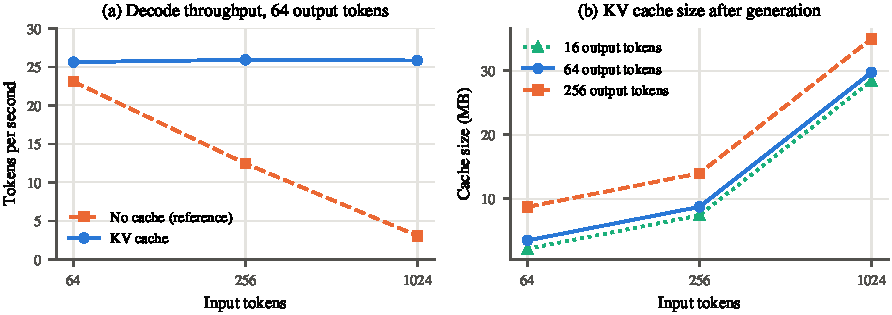
\includegraphics[width=\textwidth]{kv_cache}
\caption{KV-cache benchmark (Tesla T4, float16, greedy, EOS ignored, median of 5). (a) Decode throughput is flat with the cache and collapses without it as the prompt grows. (b) Cache size grows linearly with total tokens at 28\,KB per token, as predicted by the GQA configuration.}
\label{fig:kv}
\end{figure*}

\subsection{Tiled Attention}
Across sequence lengths 64--4{,}096, tile sizes 16--256, causal, padding and no masks, and float32/float64, the tiled implementation matched reference attention with maximum absolute error at most $1.3\times10^{-6}$ in float32 (mean about $2\times10^{-8}$), the same order as PyTorch's fused kernel. Fig.~\ref{fig:attn} shows the honest performance picture on the T4. The tiled version is slower than the reference (87.9 vs 41.9\,ms at 4{,}096 with 256-token tiles; 16.1\,s with 16-token tiles) and much slower than the fused kernel (13.9\,ms): each tile is a separate Python iteration with its own kernel launches, small allocations and interpreter overhead, whereas a fused kernel runs the same loop in on-chip memory without returning to Python. Memory is where tiling pays off: at length 4{,}096 the reference needs 1{,}536\,MB above its inputs for the score matrix, the tiled version 18.5\,MB, and even the fused kernel 72\,MB. On CPU, where there is no launch overhead and the 512\,MB score tensor stresses the cache, 256-token tiles were 5.2$\times$ faster than the reference at length 4{,}096 (390 vs 2{,}032\,ms), helped by skipping 47\% of tiles under the causal mask.

\begin{figure*}[t]
\centering
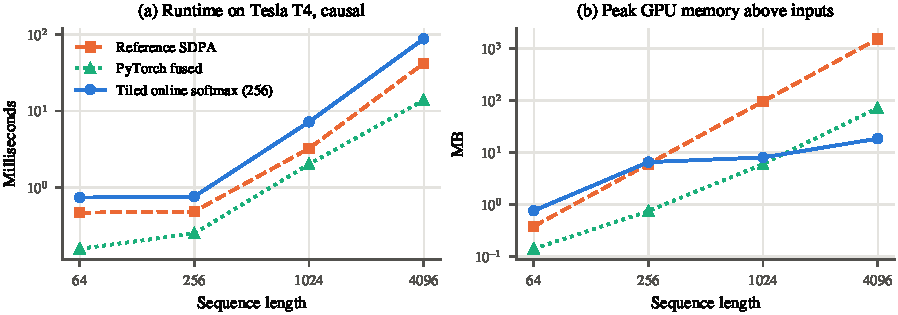
\includegraphics[width=\textwidth]{attention}
\caption{Attention benchmark on a Tesla T4 (float32, 8 heads, head dimension 64, causal mask). (a) The educational tiled implementation is slower than both the reference and the fused kernel because of per-tile Python and launch overhead. (b) It uses near-constant extra memory, whereas the reference grows quadratically to 1.5\,GB at length 4096.}
\label{fig:attn}
\end{figure*}

\subsection{Speculative Decoding}
On every prompt and every draft length the speculative output equalled greedy decoding token for token (Table~\ref{tab:spec}). Yet it was slower: 0.76--0.85$\times$ on the 20 real screening prompts and 0.51--0.77$\times$ on longer generations (Fig.~\ref{fig:spec}a). The measured breakdown explains why. For screening JSON with $k=4$, acceptance was high (90.9\%, 3.53 tokens accepted per round) and target verification took only 2.53\,s against 10.5\,s of greedy decoding, but drafting took 8.73\,s. At these model sizes and batch size 1 the T4 is latency-bound: a 0.5B forward pass costs almost as much as a 1.5B pass because fixed per-step costs (kernel launches, Python, mask construction) dominate, so the draft is not ``cheap'' in the sense the method requires \cite{leviathan2023fast}. On free-form continuations acceptance falls sharply with $k$ (Fig.~\ref{fig:spec}b; 43\% at $k=8$), so longer drafts waste more work. Fine-tuning the draft (R6) raised acceptance on screening prompts from 82.3\% to 90.9\% at $k=4$ and narrowed the slowdown from 0.76$\times$ to 0.81$\times$, but could not overcome the cost ratio. Extra memory for both caches was negligible (0.11\,GB). On the laptop, placing the draft on CPU made decoding about three times slower; on the CPU-only demonstration machine, where both models are compute-bound, the live comparison came close to break-even (12.1 vs 11.5\,s). A speedup would require a larger target, a much smaller draft, or a fused inference runtime.

\begin{table}[t]
\centering
\caption{Speculative decoding on 20 screening prompts (Tesla T4, fine-tuned draft, 288 output tokens, median of 5). All outputs equal greedy.}
\label{tab:spec}
\setlength{\tabcolsep}{3pt}
\begin{tabular}{lccccc}
\toprule
Mode & Total (s) & Tok/s & Speedup & Accept & Tok/round \\
\midrule
Greedy & 12.04 & 23.9 & 1.00 & -- & -- \\
$k=2$ & 15.83 & 18.2 & 0.76 & 97.1\% & 1.93 \\
$k=4$ & 14.90 & 19.3 & 0.81 & 90.9\% & 3.53 \\
$k=8$ & 14.23 & 20.2 & 0.85 & 90.1\% & 5.84 \\
\bottomrule
\end{tabular}
\end{table}

\begin{figure*}[t]
\centering
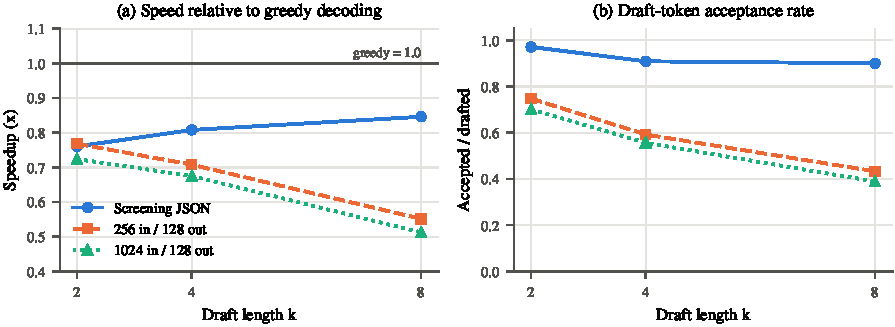
\includegraphics[width=\textwidth]{speculative}
\caption{Speculative decoding with the fine-tuned 0.5B draft on a Tesla T4. (a) Speed relative to greedy decoding stays below 1 for every scenario and draft length. (b) Acceptance is high for short, formulaic screening outputs but falls with $k$ on longer free-form generations.}
\label{fig:spec}
\end{figure*}

%=====================================================================
\section{Limitations}
%=====================================================================
The test split has only 8 patients, so intervals are wide (macro-F1 0.43--0.64) and one patient--trial pair can dominate an error cell. Rare labels are barely represented: \emph{excluded} has no test rows and cannot be evaluated, and \emph{not applicable} annotations are not internally consistent. The model's tendency to answer \emph{not excluded} without evidence is learned from the annotations themselves; the application mitigates it by flagging uncited verdicts but the model is not fixed. Explanations are templates, not reasoning, and a correct citation shows where the model looked, not that its reasoning was sound. The efficiency mechanisms are educational: tiled attention is slower than a fused kernel, and speculative decoding did not accelerate this model pair on the hardware tested. The CPU demonstration takes several seconds per criterion. Finally, the system is a research prototype evaluated against expert annotations, not a validated medical device, and must not be used for enrolment decisions.

%=====================================================================
\section{Conclusion}
%=====================================================================
A 1.5B-parameter open-weight decoder, adapted with LoRA on 602 expert-labelled criteria, learned to produce valid, evidence-citing criterion judgements and raised held-out macro-F1 from 0.234 to 0.560 and evidence micro-F1 from 0.130 to 0.523, while preserving the uncertain and not-applicable categories. Explicit implementations confirmed the textbook behaviour of three inference techniques and their practical limits: KV caching is exact and removes the quadratic slowdown; tiled online-softmax attention is exact to $10^{-6}$ and turns quadratic memory into near-constant memory but needs kernel fusion for speed; greedy speculative decoding is exact but only helps when drafting is far cheaper than verification. Future work should add consistent annotations for rare labels, calibrated abstention, and fused inference kernels.

\section*{Reproducibility}
Source code, environment files, the split manifest, training logs, predictions, metrics and benchmark logs are at \url{https://github.com/humaa-taj/Clinical-records-screener}. LoRA adapters are hosted at \url{https://huggingface.co/faa-tehe/crs-qwen2.5-1.5b-lora} and \url{https://huggingface.co/faa-tehe/crs-qwen2.5-0.5b-draft-lora} at pinned revisions and fetched by \code{scripts/setup\_env.sh}. Figures are regenerated from committed results with \code{scripts/make\_figures.py}. The demonstration video is at: \textit{[add link]}.

\appendices
\section{Use of AI Assistants}
AI coding assistants (Anthropic Claude) were used to help write and refactor code, set up the repository and environment, design the web interface, generate figures from committed results, and draft parts of this report. All model training, evaluation and benchmarking were executed by the author, and every reported number is read from the committed result files. Reused or generated code is covered by the project's test suite (252 tests), and the author reviewed and can explain every component. No GPT-4 output from the dataset was used as model input, training target or evaluation reference.

\bibliographystyle{IEEEtran}
\bibliography{refs}

\end{document}
